% !Mode:: "TeX:UTF-8"

\chapter{SDN网络下的并行路由优化算法设计}
\section{引言}
路由优化能够有效提高网络性能,提高网络资源利用率,保障用户Qos需求,
软件定义网络是一个新兴的,将控制和数据平面分离的网络范型,在SDN网络中,控制平面被分离驻留在一个集中的网络控制器上,它提供了用于网络应用程序和控制数据平面的编程接口(使用标准协议,例如OpenFlow[1])。SDN的结构使得网络管理者可以根据网络当前情况来进行有效的在线路由优化。微软[1]和谷歌[1]的实验结果证明,在SDN网络结构的数据中心网络中,路由优化能够在网络吞吐量和链路利用率上达到接近最优化性能的表现。
但是另一方面,SDN网络下中心控制的路由优化面临大规模计算问题,第一,随着网络应用的快速增加,在SDN网络中短时间内可能会有大量业务到达控制器,所以控制平面必须短时间内为大量业务计算路由。第二,为了适应大业务量的加入,网络规模也快速增大(e.g., a data center network may have hundreds of thousands of switches [9]).因此,对大量业务的快速和高效的路由优化成为了一个重要却困难的问题。为了加快网络优化过程,减小网络延迟,本文利用GPU的大规模的并行能力来加速网络优化算法的计算过程。
对大规模业务的路由优化问题可以建模成一个多商品流问题,将网络路由业务作为输入,寻找最优的路由路径来最优化效用函数,效用函数通常设置为对网络拥塞程度的评价水平,比如,最常用的效用函数是最小化最大链路利用率(MLU),
简单地被定义为利用率最高的那条链路的链路利用率[],另外一些把所有链路的链路利用率的和作为效用函数([],[])。这些效用函数的逻辑是:(1)低链路利用率意味着低的网络延迟。(2).维持低的链路利用率意味着预留更多的空间给其他将来到达的业务。
但是大量基于实际拓扑的实验表明链路利用率效用函数,特别是链路利用率,在网络利用率没有达到拥塞程度的时候,不是对网络优化的较好评价函数[]。
在这个实验中,当链路利用率低于0.9的时候会造成不可忽略的网络性能中断。所以作为替代,文章在链路容量约束的情况下来优化路由总代价。我们假设已经知道短时间内到达的一批业务,控制器需要计算出满足链路容量约束的路径,并且最优化链路路由总代价。为了使得加入网络的业务尽量多,我们设定被阻塞的业务代价为一个较大值。本文中考虑的优化问题是一个NP-hard问题,因为他等价于一般的带整数约束的商品流问题[]。
路由优化问题是一个组合优化问题,一般来说,在大规模网络中求解路由优化问题是计算困难的,因此,为了在短时间内求解路由优化问题,很多启发式算法被提出来[]。然而,大部分算法都是单线程的串行算法,串行算法的复杂度随着网络规模大小呈指数上升,SDN网络下的在线路由优化要求很短的路由优化时间,为了加速算法,一个很自然的选择就是设计并行优化算法,采用大量的线程同时计算路由路径。
本章主要设计两种路由优化算法,第一种是基于备选路径选择的路由优化算法,采用遗传算法来优化目标函数,并且设计了遗传算法的并行版本,获得几十倍的加速比,第二种是基于拉格朗日松弛的优化算法,算法把链路容量约束松弛到目标函数,并把路由优化问题分解成一堆路由路径计算问题,从而采用GPU进行并行计算。

\section{网络模型和问题建模}
\subsection{网络模型}
本文将SDN网络建模成无向图 $G(V, E)$,$V$表示所有的点集合, $E$是所有边的集合, $n = |V|$ 和 $m = |L|$分别表示点数和边数。对每一条边$(i,j)\in E$, $w_{ij}$表示此边 $(i,j)$上的权重(传输一单位的流量需要的代价),不失一般性,我们假设每条链路上的$w_{ij}$是整数,对每一条边 $(i,j)$, $c_{ij}$表示此边上的容量,假设$D$表示需要被路由的业务需求集合,业务$d \in D$是一个元组 $(s_d, t_d, bw_d)$,其中, $s_d$表示业务的源节点,$t_d$表示业务的目的节点,$bw_d$表示业务d需要的流量带宽。
业务量工程问题将网络业务需求和网络拓扑作为输入,计算出每条业务的路由路径以使得效用函数代价最小化,在SDN网络中,业务的路径在中心控制器上计算出来,为了满足用户业务的QoS要求,本文假设链路利用率不能超过一个固定阈值 $\theta$,因此,一些业务会因为链路上容量不足而被阻塞,本文用 $\hat{D}$来表示这些被阻塞的业务集合。
\subsection{问题建模}
本小节,我们把路由优化问题建模成一个混合整数规划模型(MILP),通常,路由优化中应用最广泛的效用函数是[][],与链路利用率成正比的,但是,最近的研究表明链路利用率不能很好的代表网络表现情况,而且一味的最求低的链路利用率,容易造成出现路由代价过大,路由跳数过长的问题,所以,本文结合了两种情况,采用新的效用函数,如下:
\begin{equation}\label{Obj1}
f(\mathbf{d})=\begin{cases}
\sum\limits_{d \in D} c(p_d) & \text{if available bandwidth is enough}\\
\sum\limits_{d \in \hat{D}} bw_{d}& \text{otherwise
}
\end{cases}
\end{equation}
其中$p_d$是计算出来的对应于业务$d$的路径,$c(p_d)$ ($c(p_d) = \sum_{(i,j)\in p_d} w_{ij}$)表示的是此路径$p_d$的代价。
因为不知道带宽是否足够容纳所有业务,(1)并不是衡量所有情况,为了衡量所有情况,我们对$G(V, E)$构建辅助图$G_a(V_a, E_a)$,初始时,让$G_a(V_a, E_a) = G(V, E)$,然后,对每个点$v \in V$ 和 $u \in V$,在$G_a(V_a, E_a)$中添加一条链路 $(v, u)$,并且设置链路 $(u,v)$的容量和代价分别为 $\infty$和 $nM$ ,其中 $M$是 $G(V, E)$中最大的链路代价,这样,$G_a(V_a, E_a)$就有足够的容量来容纳业务需求,如果某条业务被路由到$G_a(V_a, E_a)$中,那么就表示这条业务被阻塞了,加入了辅助图$G_a(V_a, E_a)$后,路由优化的效用函数可以表示为:
\begin{equation}\label{Obj2}
z^* = minimize~f(\mathbf{d})=
\sum\limits_{d \in D} c(p_d)=  \sum\limits_{d \in D}\sum\limits_{e \in p_d} w_e
\end{equation}
在路由优化问题中,每个业务只能够路由到一条路径上,以下整数约束能够保证每个业务只走一条路径
\begin{equation}\label{FlowConv}
\begin{split}
\sum\limits_{(i,j) \in E_a} x_{ij}^d - \sum\limits_{(j,i) \in E_a} x_{ji}^d
=\begin{cases}
1 & \text{if $i = s_d$}\\
-1 & \text{if $i = t_d$} \\
0 &{ohterwise}
\end{cases}
\\~~~~~~~~\forall i\in V_a, \forall d\in D
\end{split}
\end{equation}
其中 $x_{ij}^d$是一个0,1整数变量, $x_{ij}^d=1$表示业务$d$路由经过链路$(i,j)$,为了避免链路拥塞,路由路径需要满足以下的链路容量约束:
\begin{equation}\label{Capcon}
\sum\limits_{d \in D}\sum\limits_{(i,j) \in E_a} x_{ij}^d \cdot bw_d \le \theta\cdot c_{ij} ~~\forall (i,j)\in E_a
\end{equation}
在这个模型中,变量的数量随着业务量大小和网络规模大小呈指数增长,所以这个MILP模型在大规模情况下很难求解。
\section{基于遗传算法的路由优化算法}
	遗传算法是一种模拟自然进化过程搜索问题最优解的启发式算法,遗传算法模仿达尔文进化论和自然选择过程来评价挑选最优解集合,从而找寻较优化的解,遗传算法从一个代表问题的可行解的种群出发,一个种群中不同个体代表了不同的解,每个个体实际上是一个染色体,染色体携带表达当前解的信息编码,初代种群产生后,对每个染色体个体进行评价,按照适者生存,优胜劣汰的原则,使得较优的个体更有可能把自己的遗传信息传递给下一代,从而得到更优化的后代,算法过程中,对一部分基因进行变异,好的变异能够提高解的质量,增加算法的搜索空间,避免算法收敛于局部最优解。遗传算法的步骤流程图如下所示:
\begin{figure}
\setlength{\belowcaptionskip}{-0.5cm}
  \begin{center}
    {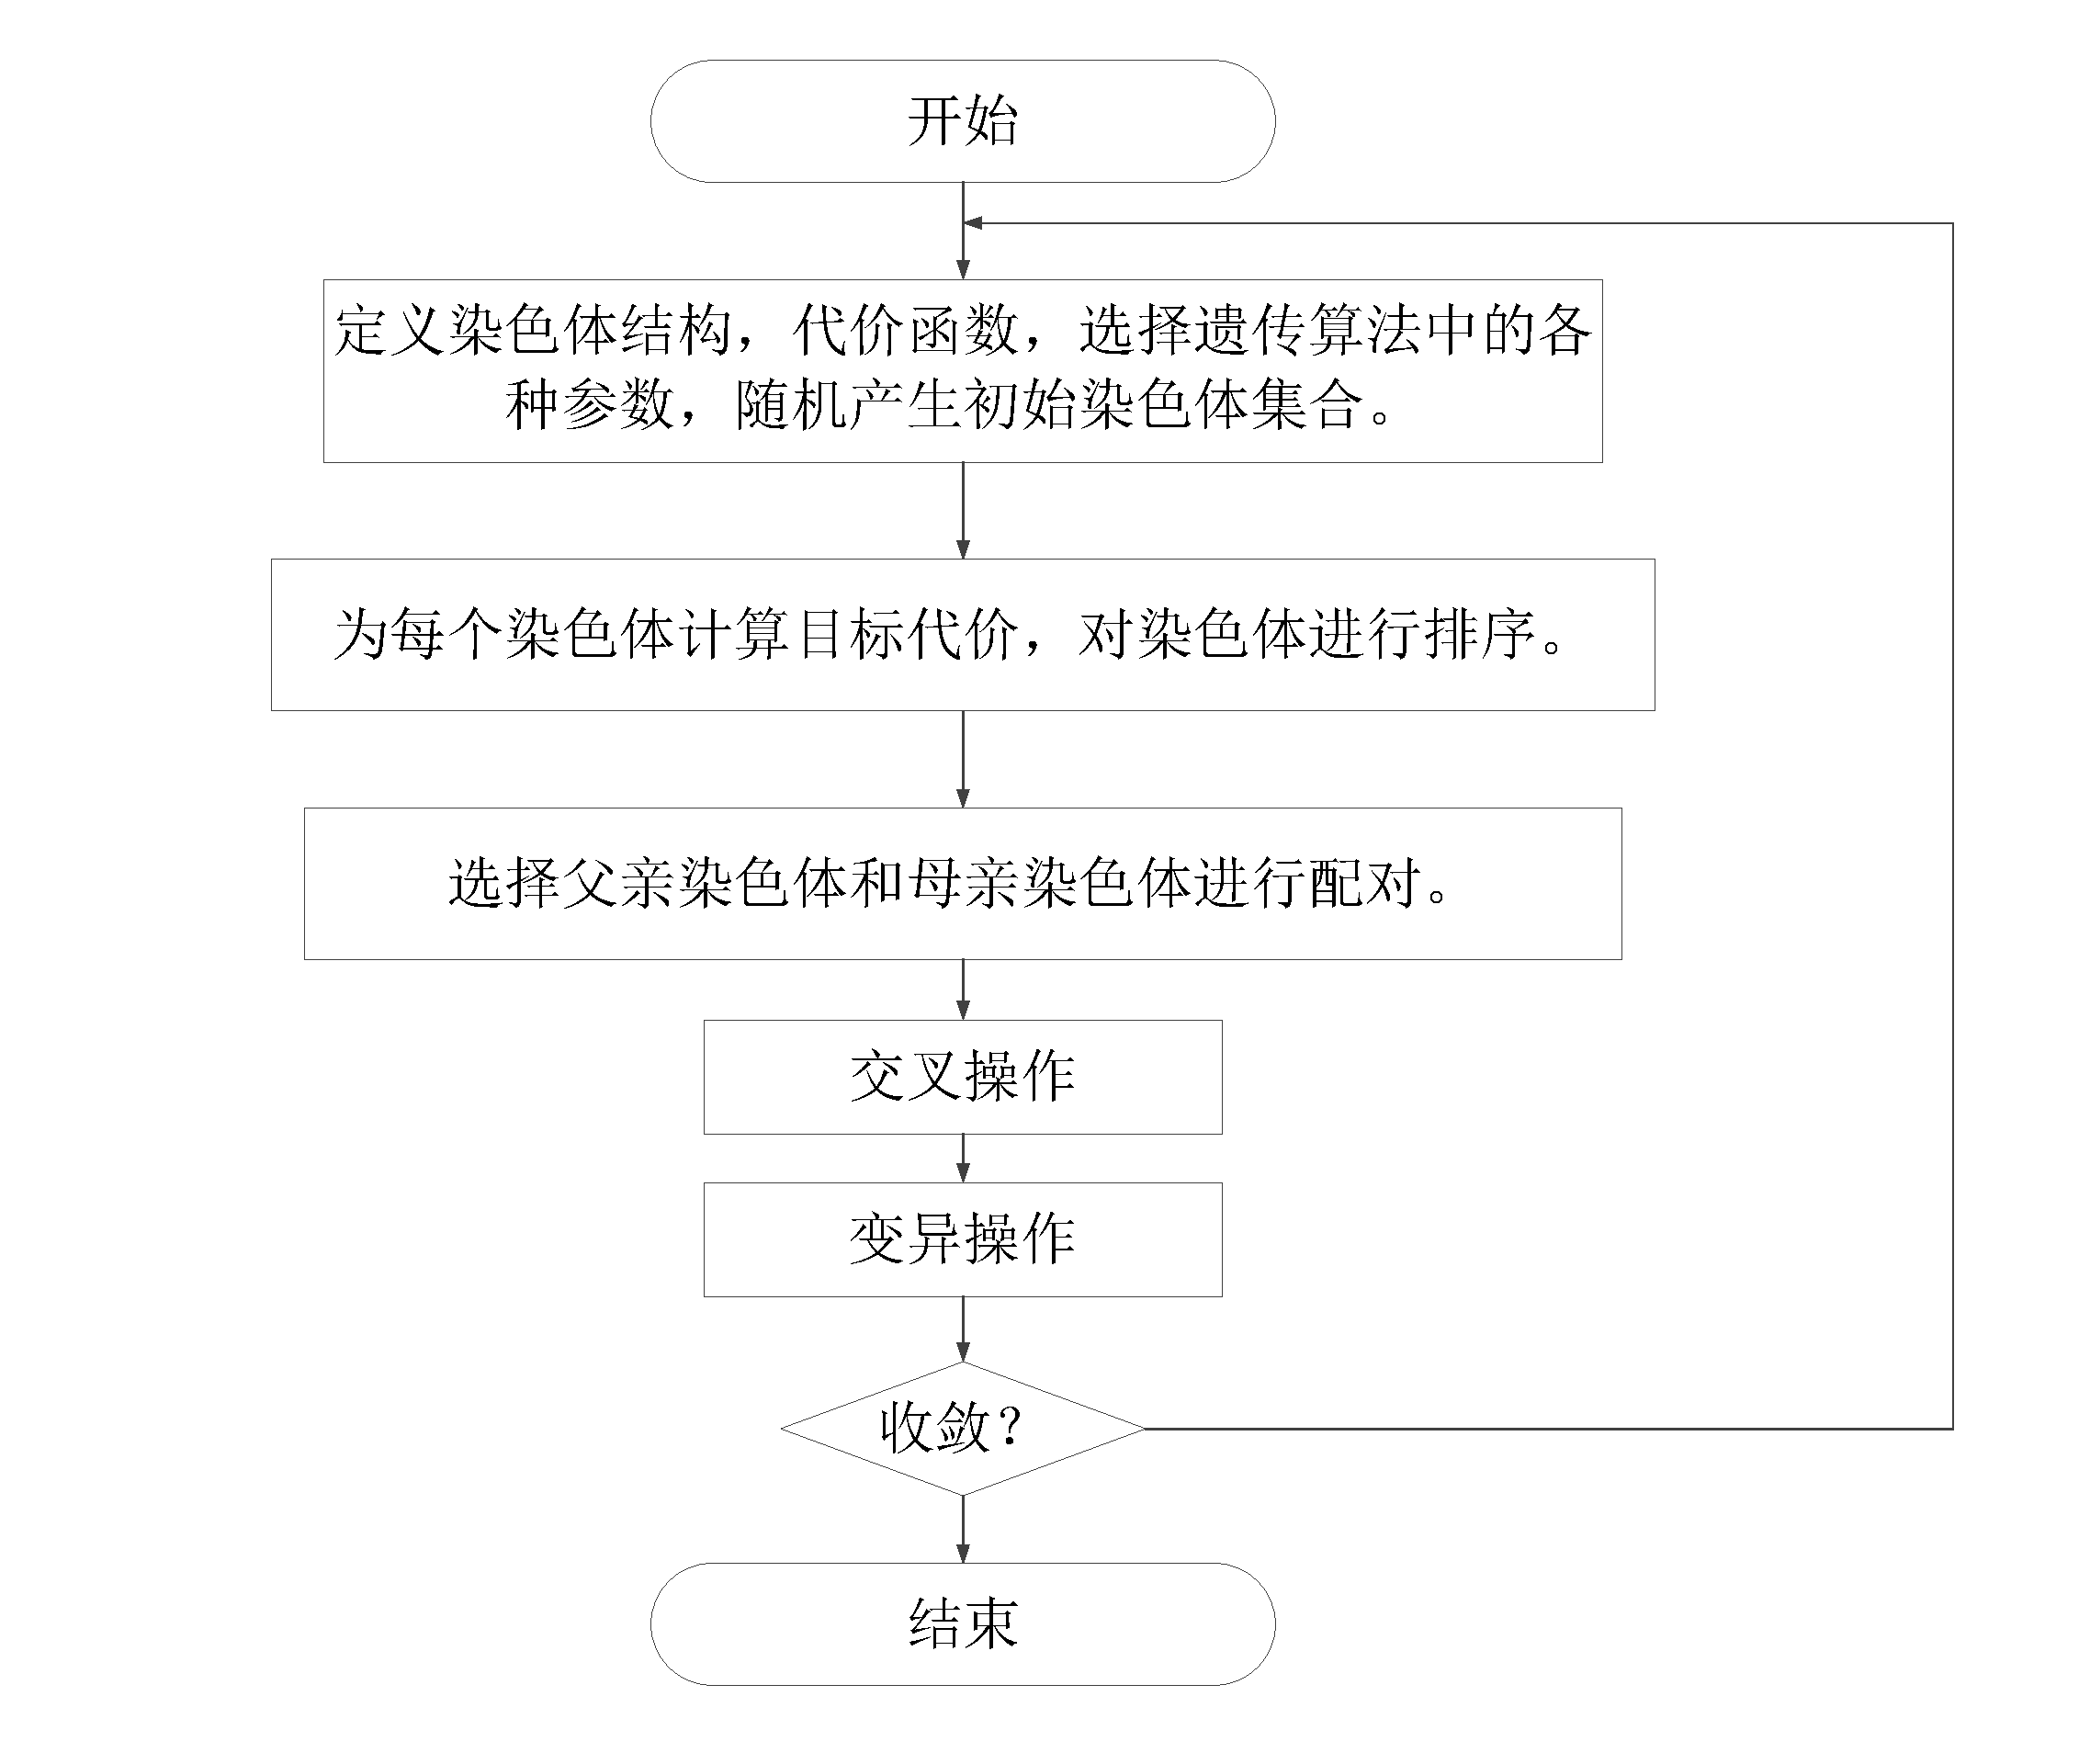
\includegraphics[width=0.45 \textwidth]{figures/GAprocess.pdf}}
    \end{center}
  \caption{{\footnotesize{GA算法流程图}}}
  \label{IterNum}
\end{figure}
\subsection{遗传算法设计}
\subsubsection{定义染色体结构}
[5][],
由前面的讨论可以知道,路由优化问题求解过程是寻找最优的业务路径集合,使得效用函数最小化,在论文[]中作者(效用函数是常见的最小化最大链路利用率)提出了一种路由优化算法,在文章中,为每一个业务$d \in D$,产生$K$条不同的备选路径作为备选路径集合$P_i={p^1_d,p^2_d,p^3_d...p^K_d}$,通过遗传算法过程来确定每个业务选择哪一条备选路径,从而找到最优解,本文采用相同的思想来求解路由优化问题,假设业务数量为$|D|$,初始染色体集合大小为$POP$对于第$j$($j in [1:POP]$)号染色体一个染色体$C_j$是一个$|D|$维数组,$C^i_j=k,k \in[1:K]$表示在第$j$号染色体中,业务$i$选择了第$k$条备选路径,$C^i_j=-1$表示业务$i$不加入网络中(在辅助图上路由),不占用链路资源,$|p^i_d|$表示业务$d$的第$i$条备选路的路径代价,$rp^i_d$表示路径$p^i_d$上的最小可用容量,$rp^i_d=min(r_e|e \in p^i_d)$,其中$e \in p^i_d$ 表示路径$p^i_d$上的边,$r_e$表示此边$e$上的剩余容量。
\subsubsection{初始可行解生成}
可行解表示满足容量约束的解,为了使得遗传算法有效,初始解的质量很重要,产生的初始解要尽量好,要有更多的业务要能加入网络中,而且保证业务的路径代价较小,文章中采用一种简单的贪心算法产生出初始可行解,算法过程如下所示:
\begin{algorithm}[htb] 
\caption{初始可行解产生} 
\label{alg:Framwork} 
\begin{algorithmic}[1] 
\Require 
$G(v,E)$:网络拓扑;
$P$:备选路径集合;
$C$:未初始化的染色体集合;  
\Ensure 
$C$:可行染色体集合; 
\For{each $c_j \in C$}
\For{each $c^d_j \in c_j$ }
\State {$c^d_j \leftarrow -1$}
\EndFor
\EndFor
\For{each $c_j \in C$}
\For{each $c^d_j \in c_j$ }
\State {$c^d_j\leftarrow k^d_j$,其中$k^d_j$为1到K之间的随机值,随机选择一条备选路}
\EndFor
\State {对染色体中的的每个业务需求按照值$\frac{bw_d}{\sqrt{|p^{k^d_j}_d|}}$}进行降序排序。
\For{each $c^d_j \in c_j$ }
\If{$rp^{k^d_j}_d>=bw_d$}
\State 加入路径$p^{k^d_j}_d$到网络,更新网络链路容量。
\Else
\State {$c^d_j \leftarrow -1$}
\EndIf
\EndFor
\EndFor
\end{algorithmic} 
\end{algorithm}
  对某一个染色体,算法随机为每个业务生成所选择的备选路径编号,但是这样选择出来的路径集合有可能会超过网络链路的容量限制,从而使得解变得不可行,要得到可行解,必须从染色体中剔除一部分业务,使得他们阻塞,为了得到比较优秀的初始可行解,本文提出一种启发式过程来确定能加入的业务,以及必须剔除的业务,一方面,要使得目标函数变小,那些流量需求较大的业务应该优先被加入到网络中,但是如果大流量的业务的路由代价很大,经过了一条很长的路径,就会大量的浪费网络中的链路容量资源,所以算法过程对当前染色体$j$中的业务和其路径按照$\frac{bw_d}{\sqrt{|p^{k^d_j}_d|}}$的值进行排序,其中${bw_d}$代表当前业务$d$所需要的流量大小,$|p^{k^d_j}_d|$代表当前染色体$j$所选择的$p^j_d$中的第${k^d_j}$条路径的代价大小。这样算法优先加入$\frac{bw_d}{\sqrt{|p^{k^d_j}_d|}}$值较大的业务,观察目标函数,目标函数是优化路由代价最小,而$\frac{bw_d}{\sqrt{|p^{k^d_j}_d|}}$较大意味着较大的流量经过较小代价的链路进行路由,这种路由是很理想的,尽量节省网络的链路使用资源的同时,又减小了总体目标函数,所以这个比例值是对业务路由个体优劣程度的较好评价,于是文章采用这个比例值来确定路径加入网络的优先级(后面第节也会应用类似的思想来调整路由),每次按照比例值排序的结果将遗传染色体所选择的路径$p^{k^d_j}_d$尝试加入到网络中,如果$rp^{k^d_j}_d>=bw_d$,表示路径经过的链路有足够的容量来容纳这一个业务,所以加入业务到网络中,并且更新网络的链路容量大小,反之,如果$rp^{k^d_j}_d<bw_d$,这个业务选择这一条路径会超过网络链路的容量限制,于是这条业务被阻塞,染色体中的相应基因位置被设置为-1。大量重复以上可行解的产生过程,则可以得到一个较好的初始染色体集合$C$。
\subsubsection{评价与交叉}
  评价过程对本轮产生的染色体,计算其相应的目标效用函数值,并且对染色体按照效用函数目标进行降序排序,由于算法过程随机交叉,可能会产生不可行的染色体解(链路容量超限),把这样的染色体评价为一个个很大的代价,从而在选优时被排除掉,目标值排在最前面的前$\alpha$个染色体为最优集合$A$,这个集合中的染色体为精英染色体,精英染色体将直接保留到下一轮迭代,此后的$\beta$个染色体为较优染色体集合$B$,较优染色体集合中的染色体不会直接保留到下一轮,但是他们有繁殖的权利,可以和精英染色体一样产生后代,遗传自己的选路信息,排在最后面的$\gamma$个染色体,组成劣等染色体集合$G$,由于其目标值一般较大,其选路策略不可取,算法直接扔掉这一部分劣等染色体,而且不让劣等染色体进行繁殖。
  交叉过程从精英染色体集合中$A$中随机选取一个染色体$c_i \in A$作为父亲,从精英染色体集合和较优染色体集合的并集$A \cup B$中随机选取一个染色体$c_j \in A \cup B$作为母亲,将$c_i$和$c_j$进行均匀交叉得到新的染色体$s$,均匀交叉过程示意如下所示,均匀交叉的过程是,对$s$的每一个基因点位以$\%50$的几率选择继承父亲或者母亲的相应点位的路径选择。重复以上过程$\beta+\gamma$次,从而产生$\beta+\gamma$个新的子染色体来替换当前染色体集合评价函数排在后$\beta+\gamma$个的染色体,因此得到新的染色体集合$C$。
\begin{figure}
\setlength{\belowcaptionskip}{-0.5cm}
  \begin{center}
    {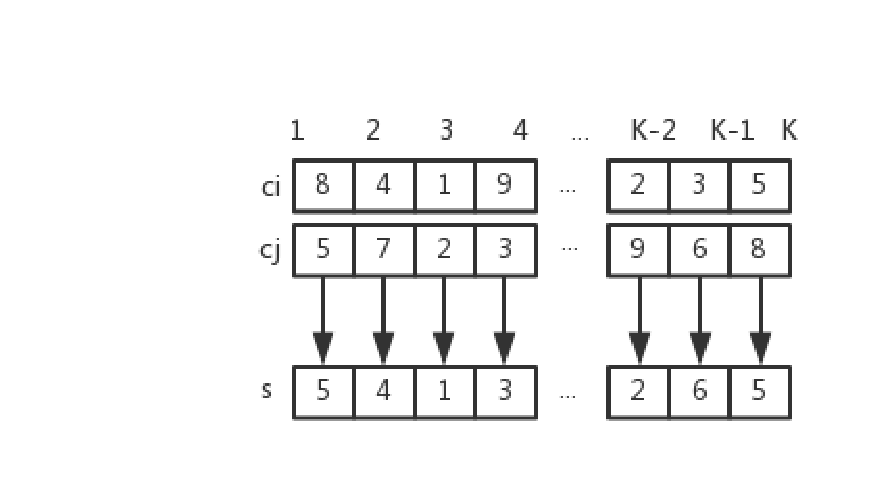
\includegraphics[width=0.45 \textwidth]{figures/cross.pdf}}
    \end{center}
  \caption{{\footnotesize{遗传算法均匀交叉过程}}}
  \label{IterNum}
\end{figure}
\subsubsection{变异与迭代终止}
  变异过程采用随机变异,随机在已经交叉后的集合$C$中选取$M \in [0:POP]$条染色体,对某一选定的染色体$c_j \in C$,随机选取$m$个业务基因点位,进行变异,将当前已经选择的路径编号随机改变为备选路集合中的另外一个值,由于变异过程是为了提高算法的的搜索空间,避免算法陷入局部最优解,但是实际实验过程中发现如果$M$和$m$值设置较大,可能使得算法收敛较慢,因为大量的变异可能会导致较优秀的可行解变成不可行,因此会丢掉这些优秀的解,因此实验中$M$和$m$的值设置得较小,变异的作用有限,算法的收敛效果主要来自于交叉步骤。
  算法每次迭代都会记录当前可行染色体解的最优目标值,如果当前迭代找到的最优可行解目标值小于全局最优值,则更新全局最优值,并且记录对应的染色体为最优解,如果迭代$L$次,全局最优值不被更新,则判定算法收敛,算法停止。
\subsection{基于GPU的并行遗传算法设计}
\subsubsection{并行评价算法设计}
  遗传算法中最消耗时间的部分是染色体评价部分,由于需要评价大量的染色体,评价每个染色体都需要大量计算开销,但是幸运的是遗传算法具有天然的并行性,每个不同的染色体评价可以并行执行,更进一步,每个染色体中的不同基因的计算也可以并行执行,这样并行粒度是很大的。
  下面将介绍评价过程的具体并行实现算法,算法主要包括可行性判断和效用函数计算两个步骤,算法计算流程如下图所示:
\begin{figure}
  \begin{center}
    {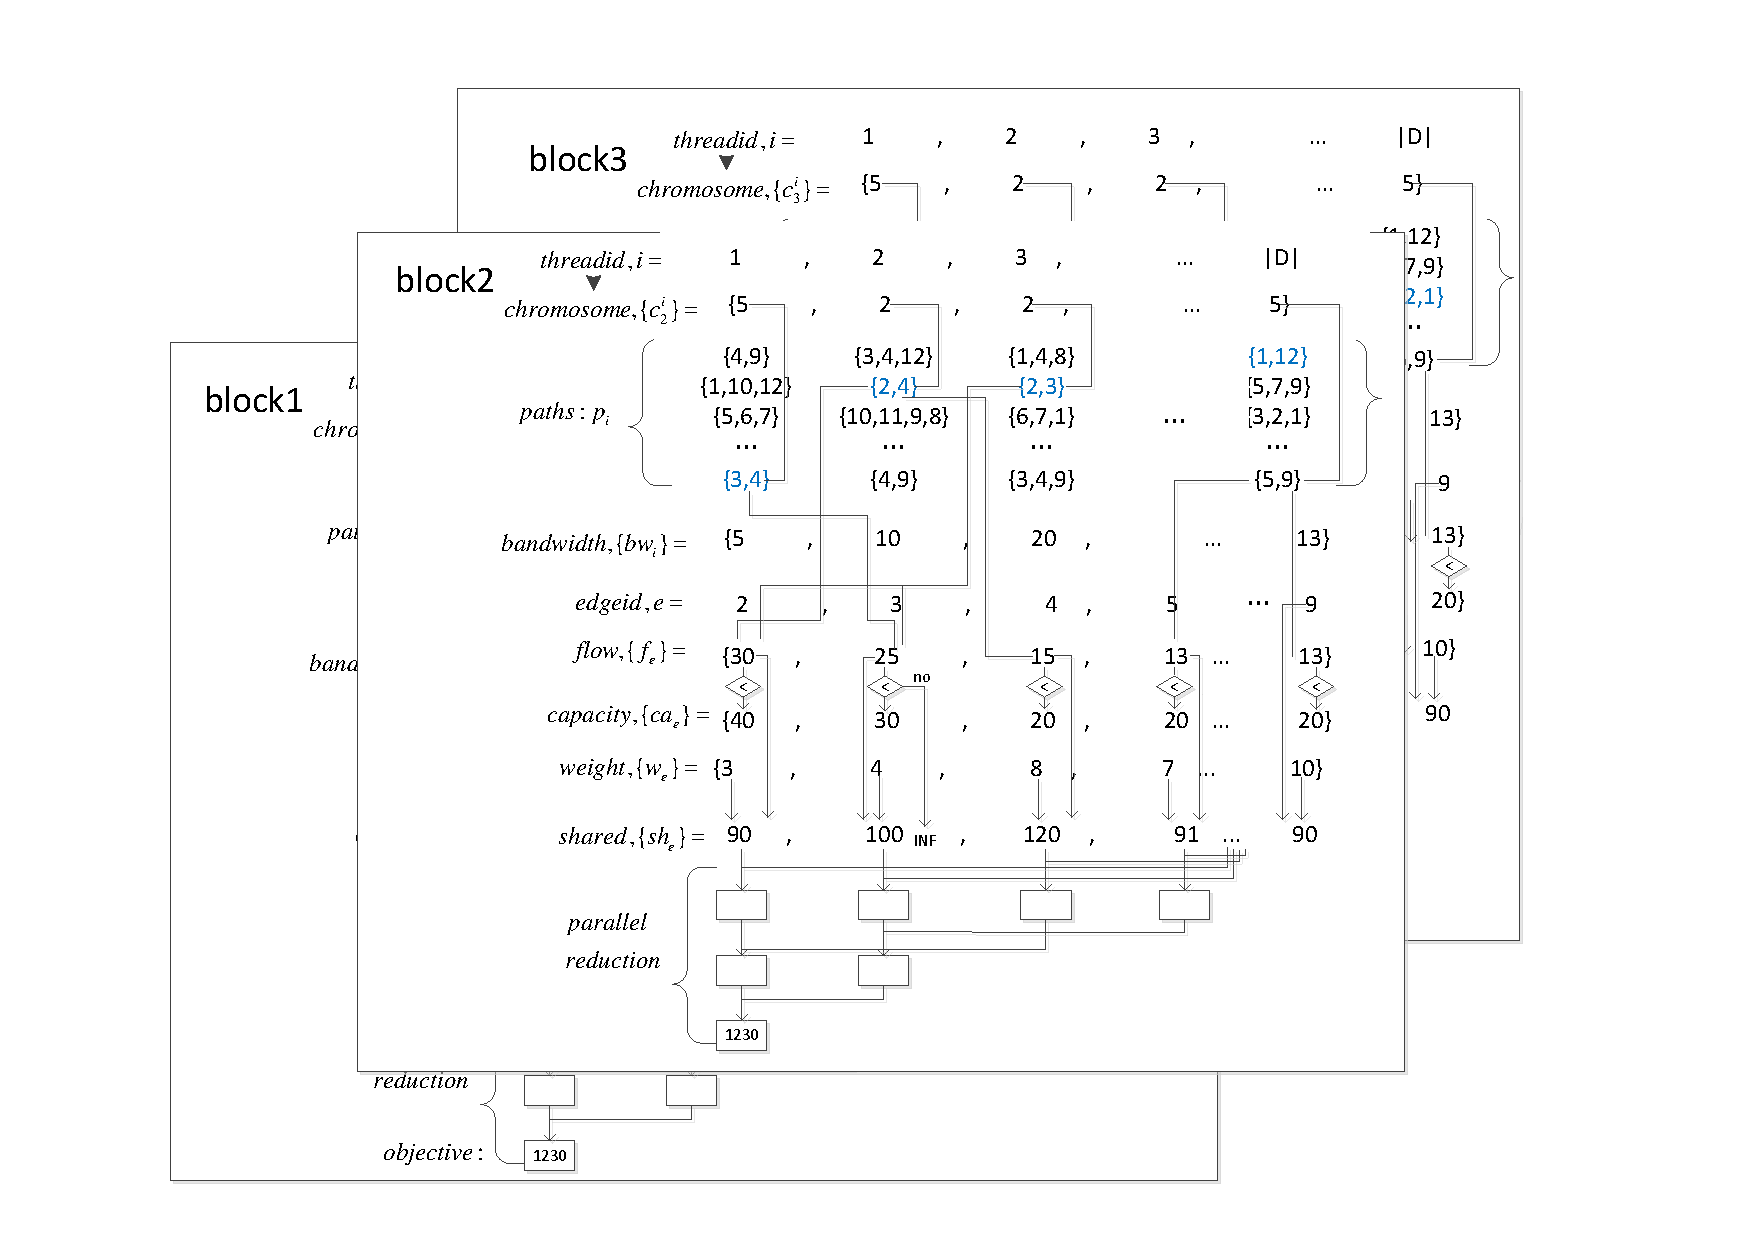
\includegraphics[width=1 \textwidth]{figures/GPUfitness.pdf}}
    \end{center}
  \caption{{\footnotesize{GPU上遗传算法评价函数计算过程图}}}
  \label{IterNum}
\end{figure}
符号解释:\newline
染色体(chromosome)基因编号:$c^d_i$表示第$i$个染色体的第$d$个基因位置。\newline
备选路径集合(paths),$p_i$表示第$i$业务的所有备选路集合。\newline
业务带宽(bandwidth),$bw_i$表示第$i$个业务需要的带宽大小。\newline
链路流量(flow),$f_e$表示第链路$e$上占用的流量大小。\newline
链路单位代价(weight),$w_e$表示链路$e$上的代价。\newline
共享内存中间数组(shared),$sh_e$表示链路$e$上的总代价。\newline
  如图所示,由于每个染色体的计算过程是独立的,算法为每一个染色体开辟一个block,每个block内部每个线程负责染色体上的相应业务,首先通过寻址备选路径集合找到这个业务选择的路径,路径上的每一个链路都需要被占用流量,于是遍历这条路径,将业务的流量加到相应的链路上,所有线程同时计算,最后得到链路上占用的流量大小为数组$flow$,并行比较$flow$和$capacity$数组,如果某一线程发现容量超限,则设置链路代价为无穷大(INF)表示此染色体不可行,最后对得到的链路代价数组进行求和,求和采用GPU上经典的并行规约算法,最后得到染色体对应的效用函数值。
  其中$flow$和$shared$两个数组被同一个block内部的线程多次访问,利用程序访问的局部性,将两个数组分配到共享内存中,这样避免了对global memery的大量慢速访问,大大提高程序计算速度。
\begin{figure}
  \begin{center}
    {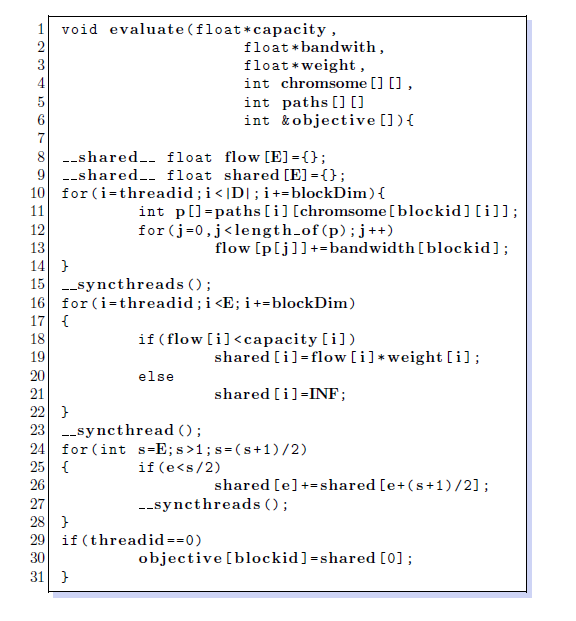
\includegraphics[width=1 \textwidth]{figures/GPUfitcode.png}}
    \end{center}
  \caption{{\footnotesize{GPU上遗传算法评价函数计算伪代码}}}
  \label{IterNum}
\end{figure}
  以上代码GPU上的评价过程伪代码,算法开始时先开辟两个大小为边数大小的共享内存数组,然后每个线程负责一个基因点,寻址基因点选择的路径,对路径上的每一条边的流量加上业务的流量大小,注意到这个时候可能同时存在多个线程访问同一个$flow$位置,所以需要同步保护,使得每个线程的加法操作都能正确执行,使用CUDA提供的atomicAdd函数来对$flow$数组进行加法操作,atomicAdd保证其调用的操作是原子操作,从而多个线程对同一$flow$位置的加法操作必修是串行执行的,一个add操作必修一次性执行完成(取址、译码、执行、访存、写回),在当前add操作执行完成之前,其他线程的add操作必修排队等待。$blockDim$表示一个block内的线程数量,代码中的for循环每次迭代标号$i$偏移$blockDim$的长度,这是因为业务量数$|D|$可能大于$blockDim$,如果这样的话,每个线程可能会负责多个业务的统计计算,每个业务标号相差$blockDim$大小。
  当线程$flow$大小统计完成之后,必修进行同步(syncthreads()),同步操作保证block内部的所有线程执行到同一步骤,也就是统计完成的线程必修等待其他统计线程都执行完成后才能继续执行,因为只有所有线程都完成对$flow$数组的加法操作,$flow$数组的统计才完整,才能够进一步进行比较操作。
  代码第19到25行计算每一条链路的路由代价,并把结果储存在$shared$数组中,如果链路上的流量小于其容量约束,那么链路代价就等于单位代价$weight$和链路流量$flow$的乘积,反之,如果流量超限,就设置$shared$为无穷大。同理,当线程计算完成后必修进行同步(syncthreads())操作,以使得shared数组正确完整。	
  为了充分利用GPU多线程,代码最后进行并行规约操作进行求和,for循环中每次将后一半的$shared$数组加到前一半,规约过程中必修进行同步(syncthreads()),以保证加法过程计算完整,最终求和值规约到一个下标0,将shared[0]中的值写入到$objective$数组中。
  另外,由于CUDA每个block支持的shared memory 大小有限,并且分配shared memory太多,会使得SIMT上的资源不足,一个block中的活跃warp数量不足,造成SIMT上不能有足够的活跃warp数量来进行切换,从而掩藏其他warp的访存延迟开销,这样会使得执行速度下降很多,所以在实际设计计算时$flow$和$shared$使用的是同一段共享内存。
\subsubsection{并行排序,变异与交叉}
  由于遗传算法中最消耗时间的部分是评价部分,本设计中对其他部分的并行步骤采用较简单的算法。
  在评价部分结束后,需要对所有的染色体按照效用函数的大小降序排序,本文采用GPU上的odd-even算法进行排序操作,odd-even算法的计算过程如下图所示:
\begin{figure}
  \begin{center}
    {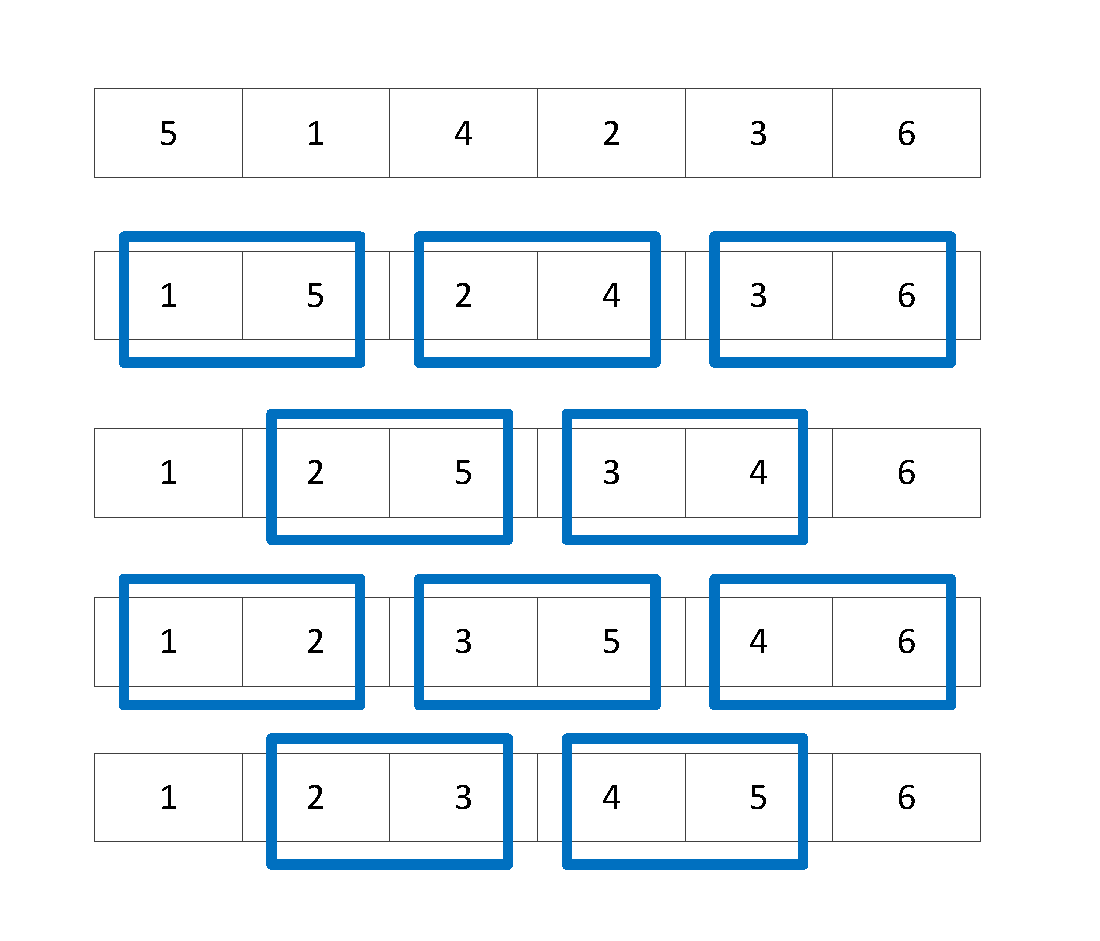
\includegraphics[width=0.8\textwidth]{figures/odd-even.pdf}}
    \end{center}
  \caption{{\footnotesize{并行奇偶排序例子}}}
  \label{IterNum}
\end{figure}
如图所示,奇偶排序算法每次两两比较数组中的值的大小,然后将较小的那个值交换到前面,奇数次的时候比较下标为$2k和2k+1$的值,其中$k \in [0,POP/2]$,偶数次的时候比较下标为$2k-1和2k$的值,其中$k \in[1,POP/2]$,最终经过$POP/2$轮的奇偶比较,就可以得到排序好的数组,从奇偶排序的执行过程可以看出,每一轮比较中的$POP/2$次比较是是相互独立无关的,其具有天然的可并行性,而且其并行实现较简单。
下面介绍染色体排序算法的GPU代码实现:
\begin{figure}
  \begin{center}
    {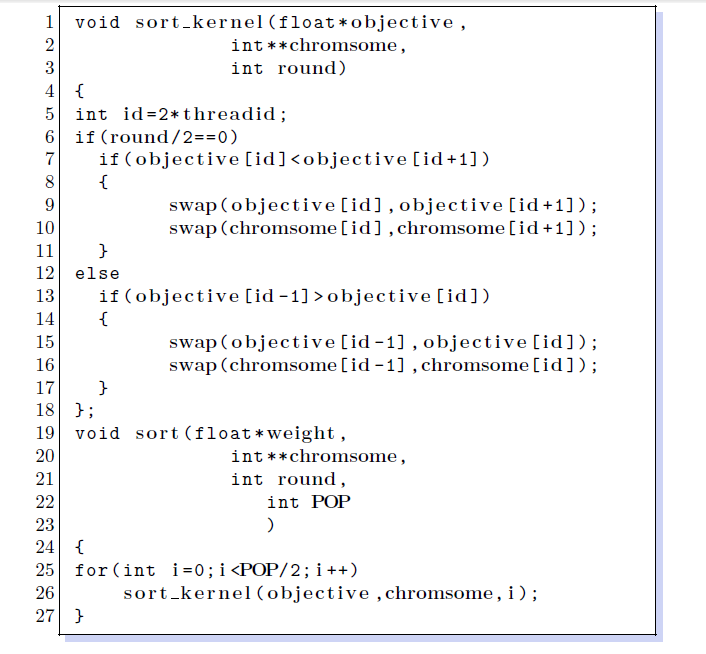
\includegraphics[width=0.8\textwidth]{figures/GPUoddeven.png}}
    \end{center}
  \caption{{\footnotesize{GPU并行奇偶排序伪代码}}}
  \label{IterNum}
\end{figure}
如图所示,sort函数一共需要执行$POP/2$轮比较,也就要调用kernel_sort$POP/2$次,在kernel_sort中,一个线程负责两个数的比较与交换操作,在寻址数组之前,要判断当前的比较轮次的奇偶性,如果为奇数,则当前标号为$threadid$的线程要去比较标号为$2*threadid$和标号为$2*threadid+1$的目标值,如果当前标号为偶数值,则去比较下标为$2*threadid-1$和$2*threadid$的值,如果出现较小的值在后面,需要进行交换操作,交换操作在交换$objective$数组的同时,也要交换相应的染色体($chromsome$)数组,这样一轮比较达到并行度为$POP/2$,一个有$POP/2$个线程参与比较交换计算,因为要循环$POP/2$次才能保证排序完毕,所以算法总的计算复杂度为$O(POP)$。
  交叉过程分为父母选取和交叉计算两个kernel,父母选取过程随机并行地选取$beta+gamma$对父母,每个线程负责选取一对父母,并且将选取的父母下标记录到$father$和$monther$数组中。
  交叉计算过程示意图如下所示:
\section{基于Lag的优化算法设计}
\subsection{问题建模}
\subsection{基于GPU的并行lag算法设计}
\subsection{仿真实验分析}
